\documentclass{beamer}
\usetheme{copenhagen}
\setbeamertemplate{headline}{}
\usepackage{graphicx}
\usepackage[utf8]{inputenc}
\usepackage{amsmath}
\usepackage{graphics}
\usepackage{xcolor}
\usepackage{listings}
\usepackage{adjustbox}
\usepackage{tikz}
\usepackage{wasysym}
\usetikzlibrary{calc,shapes, arrows, positioning, shapes.gates.ee, trees}
\usepackage{hyperref}
\usepackage{booktabs}
\usepackage{multirow}
\usepackage{enumitem}
\usepackage{array}
\usepackage{longtable}
\usepackage{verbatim}
\newlist{bracketedromanenum}{enumerate}{1}
\setlist[bracketedromanenum]{
	label={(\roman*)},
	ref={\roman*},
	itemsep=0.5em,
	topsep=0.5em
}

\title{FACTOR ANALYSIS}

\begin{document}
	\maketitle
\section{INTRODUCTION}

\begin{frame}{Introduction}
	$\bullet$ Factor Analysis is a statistical technique used to uncover the underlying sections or dimensions within a set of observed variables. \\
	\vspace{0.2cm}
	$\bullet$ The allure of Factor analysis over other approaches to the study of hypothetical constructs is its capacity of testing detailed hypothesis in a inferential mode.\\
	\vspace{0.2cm}
 $\bullet$ Factor extraction involves identifying the underlying factors by examining the pattern of correlations among the observed variables which can be done using Principal Component Analysis (PCA).\\
	\vspace{0.2cm}
$\bullet$ Once the factors are extracted, researchers employ factor rotation techniques (varimax, oblique rotation) to simplify the interpretation of the factor structure.
\end{frame}

\begin{frame}{Statement of problem}
$\bullet$ Many reseachers in psychology and social science are forced with the problem of comparing latent constucts that are not directly observable.\\
	
\vspace{0.4cm}
	
$\bullet$ Factory Analysis has become the standard to identify and interpret these underlying constructs.\\
\vspace{0.4cm}

\underline{\textbf{Specific objective}}\\

$\bullet$  To identify the latent factors contributing to presence and severity of depression.\\
\vspace{0.4cm}
$\bullet$ To assess the reliability of the Factor model in explaining depression severity.	
\end{frame}

\section{Literature Review}
\begin{frame}{Literature Review}
$\bullet$ Let's review some key concepts from previous research perspectives that have
contributed to recent advances in mental health understanding and then presents the implications of this knowledge for accurate screening of major depressive disorder.\\
\vspace{3mm}
$\bullet$ Jain et al. (2013) examined the burden of depression on work productivity in the US workforce. The Patient Health Questionnaire for depression severity and the Health and Work Performance Questionnaire and Work Productivity and Activity Impairment (WPAI) Questionnaire for absenteeism and presenteeism were used to survey 1051 full-time employees in February 2010.\\
\vspace{3mm}
$\bullet$ All levels of depression were associated with decreased work productivity as severity increased, presenteeism and absenteeism worsened.
\end{frame}


\begin{frame}{Cont...}
$\bullet$ In another study Serpa et al. (2014), investigated the major problems among Veterans
specifically anxiety, depression and suicidal ideation. \\
\vspace{3mm}
$\bullet$ Pre- and Post Mindfulness Based Stress Reduction (MBSR) questionnaires were used to collect data on MBSR’s effectiveness among 79 veterans at an urban Veterans Health Administration medical facility and were used for comparison among individuals. \\
\vspace{3mm}
$\bullet$ The results indicated significant reductions in anxiety, depressions, and  suicidal ideation after MBSR training as well as improved mental health functioning scores although pain intensity and physical health functionality did not register improvements
\end{frame}

\section{Methodology}
\begin{frame}{Factor Analysis Model}

$\bullet$ The general model of a Factor analysis is, (Johnson and Wichern, 2007)
\begin{equation}
	\begin{gathered}
		X_1-\mu_1=\ell_{11} F_1+\ell_{12} F_2+\cdots+\ell_{1 m} F_m+\varepsilon_1 \\
		X_2-\mu_2=\ell_{21} F_1+\ell_{22} F_2+\cdots+\ell_{2 m} F_m+\varepsilon_2 \\
		\vdots \\
		\vdots \\
		X_p-\mu_p=\ell_{p 1} F_1+\ell_{p 2} F_2+\cdots+\ell_{p m} F_m+\varepsilon_p
	\end{gathered}
\end{equation}

\vspace{2mm}
	or in matrix notation
	\begin{equation}
		\mathbf{X}- \boldsymbol{\mu}=\mathbf{L}\mathbf{F}+ \boldsymbol{\varepsilon}
	\end{equation}
\end{frame}

\begin{frame}{Covariance Structure for the  Factor Model}
$\bullet$ The Factor model implies a covariance structure for $\mathbf{X}$.
	
	$$Cov(\mathbf{X)=LL'} +\Psi$$ 
	
	and
	
	$$Cov(\mathbf{X,F})= \mathbf{L}$$
\begin{equation}
	\underbrace{\sigma_{ii}}_{Var(X_i)}= \underbrace{\ell_{i1}^2 + \ell_{i2}^2 + \cdots + \ell_{im}^2}_\text{Communality} +\underbrace{\psi_i}_\text{Unique variance}
\end{equation}
\end{frame}
\subsection{Factor Extraction}
\begin{frame}{Principal Component Solution of the Factor Model}
$\bullet$ The goal of a PCA is to replicate the correlation matrix using a set of components that are fewer in number and linear combinations of the original set of items. \\
The matrix of estimated factor loadings $\left\{\tilde{\ell}_{i j}\right\}$ is given by;
	\begin{equation}
		\tilde{\mathbf{L}}=\left[\sqrt{\hat{\lambda}_1} \hat{\mathbf{e}}_1: \sqrt{\hat{\lambda}_2} \hat{\mathbf{e}}_2: \cdots: \sqrt{\hat{\lambda}_{\mathrm{m}}} \hat{\mathbf{e}}_{\mathrm{m}}\right]
	\end{equation}\\
\vspace{2mm}
\textbf{How, then, do we select the number of factors $m$?}\\

$\bullet$ The number of common factors retained in the model is increased until a ”suitable proportion” of the total sample variance has been explained.

$\bullet$ After deciding on the number of factors to extract and with analysis model to use, the next step is to interpret the factor loadings then we conduct Factor rotations help us interpret factor loadings.
\end{frame}
\section{Data Analysis and Results}
\begin{frame}{Variable Description}
$\mathbf{x_1<-}$Little interest or pleasure in doing things.\\
$\mathbf{x_2<-}$ Feeling down, depressed, or hopeless.\\
$\mathbf{x_3<-}$Trouble falling or staying asleep, or sleeping too much.\\
$\mathbf{x_4<-}$Feeling tired or having little energy.\\
$\mathbf{x_5<-}$Feeling bad about yourself -or that you are a failure or have let yourself or your family down.\\
$\mathbf{x_6<-}$Moving or speaking so slowly that other people could have noticed? Or the opposite.\\
$\mathbf{x_7<-}$Trouble concentrating on things, such as reading the newspaper or watching television\\
$\mathbf{x_8<-}$Poor appetite or overeating\\
$\mathbf{x_9<-}$Thoughts that you would be better off dead or hurting yourself in some way.
\end{frame}

\begin{frame}{First Ten Observation}
	
\begin{longtable}[t]{|rrrrrrrrrrrr|}
		\toprule
	Index & Gender & Age & x1 & x2 & x3 & x4 & x5 & x6 & x7 & x8 & x9\\
	\midrule
	1 & 2 & 22 & 1 & 2 & 1 & 1 & 1 & 3 & 2 & 1 & 0\\
	2 & 1 & 35 & 3 & 1 & 1 & 1 & 2 & 2 & 0 & 2 & 0\\
	3 & 2 & 22 & 1 & 1 & 1 & 2 & 3 & 2 & 0 & 1 & 1\\
	4 & 1 & 25 & 1 & 1 & 1 & 1 & 0 & 3 & 1 & 1 & 0\\
	5 & 1 & 24 & 3 & 2 & 3 & 0 & 3 & 3 & 1 & 1 & 3\\
	\addlinespace
	6 & 1 & 24 & 1 & 1 & 1 & 0 & 0 & 1 & 0 & 0 & 0\\
	7 & 2 & 25 & 3 & 1 & 1 & 2 & 1 & 1 & 1 & 2 & 0\\
	8 & 2 & 20 & 1 & 3 & 2 & 1 & 0 & 3 & 1 & 1 & 0\\
	9 & 2 & 20 & 3 & 1 & 0 & 1 & 0 & 1 & 1 & 0 & 0\\
	10 & 2 & 24 & 1 & 1 & 0 & 3 & 1 & 1 & 0 & 1 & 0\\
	\bottomrule
\end{longtable}	

\end{frame}

\begin{frame}{Factor Extraction}

\begin{columns}[c]
\begin{column}{0.5\textwidth}


\includegraphics[scale=0.5]{Rplot01.pdf}
\end{column}

\begin{column}{.4\textwidth}
\textbf{How do we choose the number of factors?}\\
One of the criterion discussed in our methodology is to choose components that have eigenvalues greater than 1.
\end{column}

\end{columns}

\end{frame}
\begin{frame}
But is does 1 factor sufficiently represent our data?

\begin{columns}[c]
	\begin{column}{0.5\textwidth}
		
		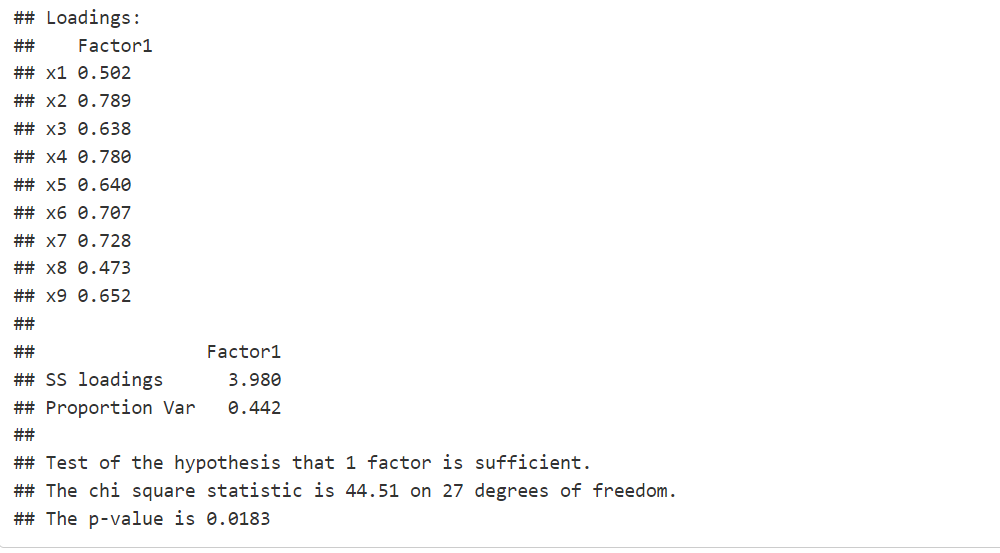
\includegraphics[scale=0.5]{Rplot02.png}
	\end{column}
	
	\begin{column}{.5\textwidth}
 $\bullet$ From the results we reject the Null.\\
 
 $\bullet$ But, when choose 2 factors we get a good fit.
	\end{column}
	
\end{columns}
\end{frame}

\begin{frame}{Factor Rotation}
\begin{columns}[c]

\begin{column}{0.5\textwidth}
	
	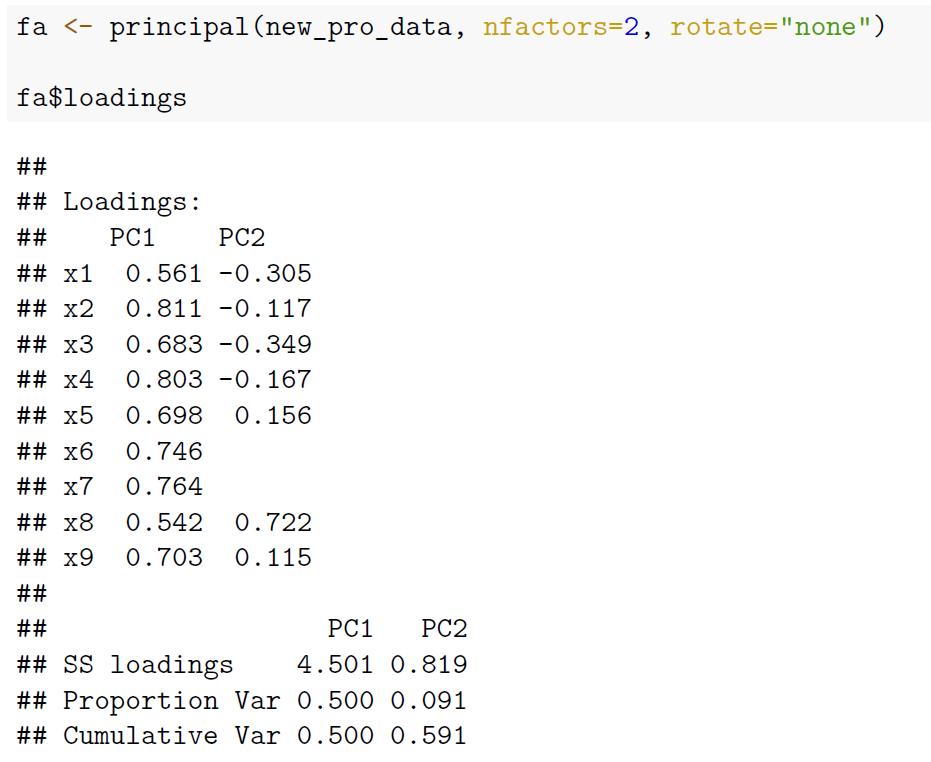
\includegraphics[scale=0.5]{Rplot04.png}
\end{column}

\begin{column}{.5\textwidth}

\end{column}

\end{columns}

\end{frame}

\begin{frame}
	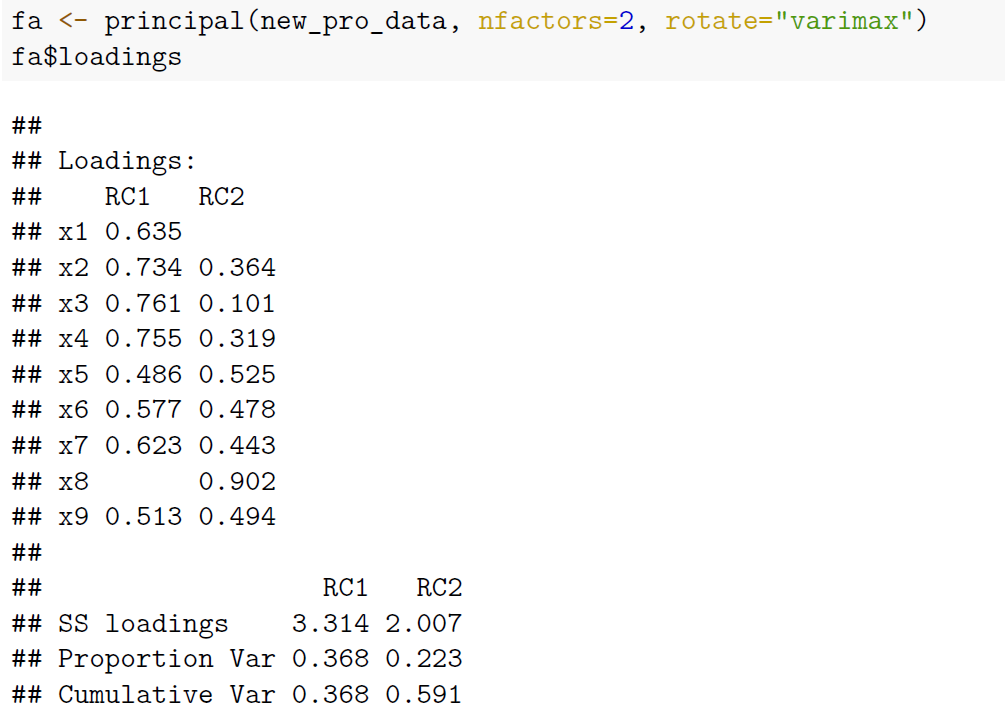
\includegraphics[scale=0.4]{Rplot03.png}
\end{frame}

\begin{frame}{Conclusions}
	$\bullet$The application of factor analysis to the Depression Severity Questionnaire administered to the Kenyan youth population has provided valuable insights into the underlying latent constructs of depression severity. \\
\vspace{3mm}	
	$\bullet$ The results of factor analysis provide evidence of the questionnaire's reliability and validity in assessing depression severity in the Kenyan context. The identification of these latent constructs enhances the questionnaire's utility as a valuable tool for future research, clinical assessments, and mental health interventions focused on Kenyan youth.\\
\end{frame}
\begin{frame}{Recommendation}
	

	$\bullet$	Refine and validate the identified latent constructs: Further validation studies should be conducted to confirm the identified latent constructs and ensure their stability and generalizability across different samples within the Kenyan youth population. \\
	
	
	
	$\bullet$ Conduct longitudinal studies: Undertake longitudinal studies to examine the stability and trajectories of the identified latent constructs over time. This will provide a deeper understanding of how depression severity evolves among Kenyan youth and inform the development of preventive strategies and early interventions.
	
\end{frame}
	


\begin{frame} {References}
	$\bullet$ Jain G., Roy A., Harikrishnan V., Yu S., Dabbous O. and Lawrence, C. (2013), Patient-Reported Depression Severity Measured by the PHQ-9 and Impact on Work Productivity, \emph{Journal of Occupational and Environmental Medicine}, 55(3), 252-258.\\
	
	$\bullet$ Johnson R.A. and Wichern D.W.,Applied Multivariate Statistical Analysis, Pearson Education, Inc., 2007.\\
	
	$\bullet$ Serpa J. G., Taylor S. L. and Tillisch K. (2014), Mindfulness-Based Stress Reduction (MBSR) Reduces Anxiety, Depression, and Suicidal Ideation in Veterans, \emph{Medical Care}, 52(12), S19-S24.
	
\end{frame}

\end{document}